\documentclass[11pt]{article}

% Packages
\usepackage[margin=1in]{geometry}
\usepackage{amsmath, amssymb}
\usepackage{graphicx}
\usepackage{caption}
\usepackage{subcaption}
\usepackage{enumitem}
\usepackage{hyperref}
\usepackage{fancyhdr}
\usepackage{titlesec}
\usepackage{xcolor}
\usepackage{float}
\usepackage{graphicx}
\usepackage{subcaption}

% Header/Footer
\pagestyle{fancy}
\fancyhf{}
\rhead{ML Project Report}
\lhead{Jonas Gericke \& Yexuan Wang}
\cfoot{\thepage}

% Section formatting
\titleformat{\section}{\large\bfseries}{\thesection}{1em}{}
\titleformat{\subsection}{\normalsize\bfseries}{\thesubsection}{1em}{}

% Title
\title{\textbf{Efficient Algorithms for Lasso Regression}}
\author{Jonas Gericke \& Yexuan Wang \\
Applied Machine Learning in Python -- LMU Munich \\
\texttt{jonas.gericke@campus.lmu.de \& yexuan.wang@campus.lmu.de}}
\date{July 15, 2025}

\begin{document}


\maketitle

\section{Task Overview and Methods}

This project investigates solving Lasso regression using two optimization methods: SubGradient Descent and ISTA (Iterative Shrinkage-Thresholding Algorithm). The primary goal is to compare their performance in terms of convergence speed, sparsity of the solution, and sensitivity to initialization and hyperparameters. Experiments were conducted on both synthetic data and the Boston Housing dataset, exploring various initialization strategies, learning rates, and regularization strengths $\lambda$.
\emph{SubGradient Descent} is simple and widely applicable, but tends to converge slowly and may produce less sparse solutions.
\emph{ISTA} on the other hans is a Proximal Gradient Descent method that incorporates soft-thresholding through proximal updates, leading to faster convergence and sparser results.
We highlights the trade-off between algorithmic simplicity and optimization efficiency in sparse regression.

The standard Lasso objective function is:
\[
    \min_{\mathbf{w}} \; \frac{1}{2n} \sum_{i=1}^n (y_i - \mathbf{x}_i^\top \mathbf{w})^2 + \lambda \|\mathbf{w}\|_1
\]

The corresponding optimization updates are:

\begin{itemize}
    \item \textbf{SubGradient update:}
          \[
              \mathbf{w}^{(t+1)} = \mathbf{w}^{(t)} - \eta \left( \nabla \ell(\mathbf{w}^{(t)}) + \lambda \cdot \text{sign}(\mathbf{w}^{(t)}) \right)
          \]

    \item \textbf{ISTA update:}
          \[
              \mathbf{w}^{(t+1)} = \text{prox}_{\eta \lambda} \left( \mathbf{w}^{(t)} - \eta \nabla \ell(\mathbf{w}^{(t)}) \right), \quad
              \text{prox}_{\eta \lambda}(z_j) = \text{sign}(z_j) \cdot \max(|z_j| - \eta \lambda, 0)
          \]

\end{itemize}

\vspace{1em}
In addition, we explored \emph{Elastic Net}, which combines Lasso and Ridge regression by adding both $\ell_1$ and $\ell_2$ regularization terms. This encourages sparsity while improving stability when features are highly correlated:
\[
    \min_{\mathbf{w} \in \mathbb{R}^d} \; \frac{1}{2n} \left\| \mathbf{Xw} - \mathbf{y} \right\|_2^2 + \lambda_1 \left\| \mathbf{w} \right\|_1 + \lambda_2 \left\| \mathbf{w} \right\|_2
\]

\subsection*{Implementation Notes}
We used fixed learning rates and iteration numbers. ISTA is expected to converge faster and yield sparser solutions, which is confirmed in our experiments.
\section{Experiments and Results}

\subsection{Training Loss and Sparsity}
Firstly, we compare SubGradient Descent and ISTA for solving the Lasso regression problem on a synthetic dataset with sparse ground truth. Using fixed \( \lambda = 0.5 \) and learning rate \( 10^{-4} \), we track training loss and sparsity over 10{,}000 iterations. ISTA shows faster convergence and better sparsity than SubGradient, consistent with theoretical expectations.

\subsection{Path behavior}
Beyond loss and sparsity metrics, we analyze the evolution of model coefficients during training.
We consider two initialization schemes: random Gaussian and all-zero initialization. With both of initial value, ISTA quickly drives many coefficients to zero, demonstrating strong sparsity-inducing behavior due to its soft-thresholding mechanism. In contrast, SubGradient Descent reduces the magnitudes of coefficients more slowly.

\begin{figure}[H]
    \centering
    \begin{subfigure}[t]{0.23\textwidth}
        \centering
        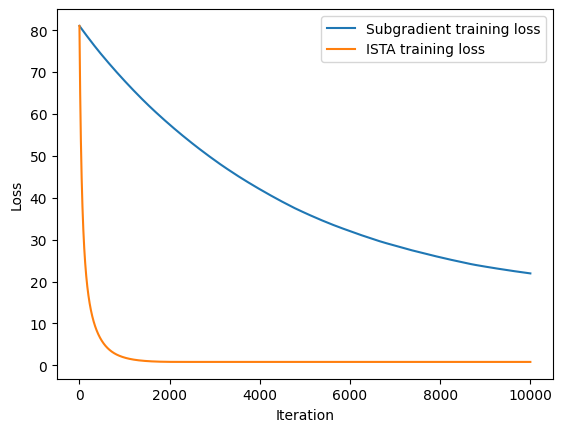
\includegraphics[width=\textwidth]{figures/fig1.png}
        \caption{2.1 Training loss of SubGradient vs. ISTA}
    \end{subfigure}
    \hfill
    \begin{subfigure}[t]{0.23\textwidth}
        \centering
        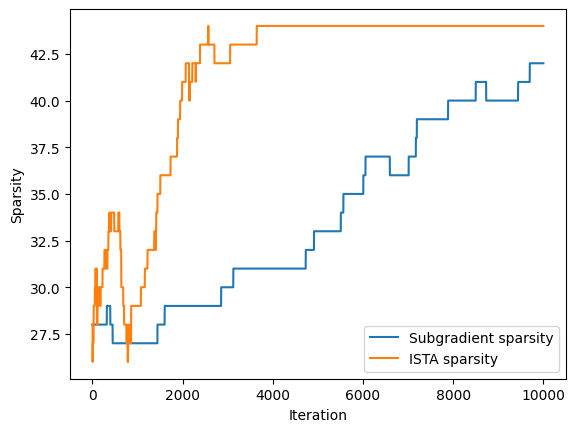
\includegraphics[width=\textwidth]{figures/fig2.png}
        \caption{2.2 Sparsity evolution of SubGradient vs. ISTA}
    \end{subfigure}
    \hfill
    \begin{subfigure}[t]{0.23\textwidth}
        \centering
        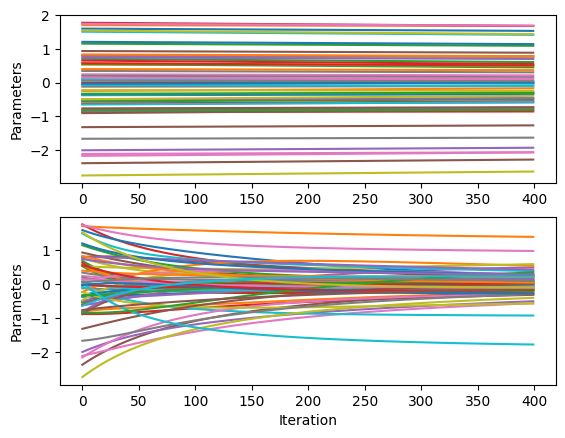
\includegraphics[width=\textwidth]{figures/fig3.png}
        \caption{2.3 Parameter paths with Gaussian initialization}
    \end{subfigure}
    \hfill
    \begin{subfigure}[t]{0.23\textwidth}
        \centering
        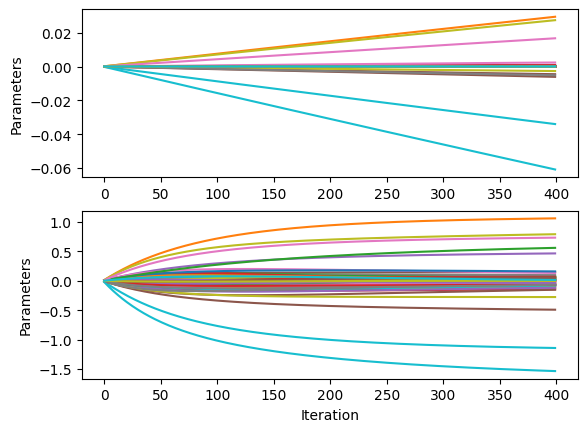
\includegraphics[width=\textwidth]{figures/fig4.png}
        \caption{2.4 Parameter paths with zero initialization}
    \end{subfigure}

    % \caption{All four subfigures in one row}
    \label{fig:four-in-a-row}
\end{figure}

\subsection{Effect of different $\lambda$ on Sparsity}
The regularization parameter \( \lambda \) controls model sparsity in Lasso. Larger values lead to stronger penalties and sparser solutions.
ISTA shows a clear increase in sparsity as \( \lambda \) grows, remaining stable and close to maximum sparsity. In contrast, SubGradient Descent fluctuates and maintains lower sparsity, indicating ISTA is more effective at enforcing regularization.

\subsection{Sensitivity to Initialization}

Initialization significantly influences the convergence behavior of optimization algorithms. We compare three strategies for  $\mathbf{w}_0$: zero initialization, random Gaussian initialization, and the least-squares solution \( \mathbf{w}_0 = (\mathbf{X}^\top \mathbf{X})^{-1} \mathbf{X}^\top \mathbf{y} \). The results show that ISTA consistently converges to highly sparse solutions regardless of initialization, demonstrating strong robustness. In contrast, SubGradient Descent is more sensitive, especially with random initialization, leading to less stable sparsity patterns.

\subsection{Convergence with Learning Rate}

To examine the effect of learning rate, we evaluate both SubGradient Descent and ISTA under a range of learning rates from 0.0001 to 0.006.
As shown in the figure, ISTA exhibits stable and consistently low error across all learning rates, indicating strong robustness to this parameter. In contrast, SubGradient Descent is much more sensitive: at low learning rates it converges slowly with high residual error, and although the error decreases with increasing learning rate, it remains significantly higher than ISTA.

\begin{figure}[H]
    \centering
    \begin{subfigure}[t]{0.32\textwidth}
        \centering
        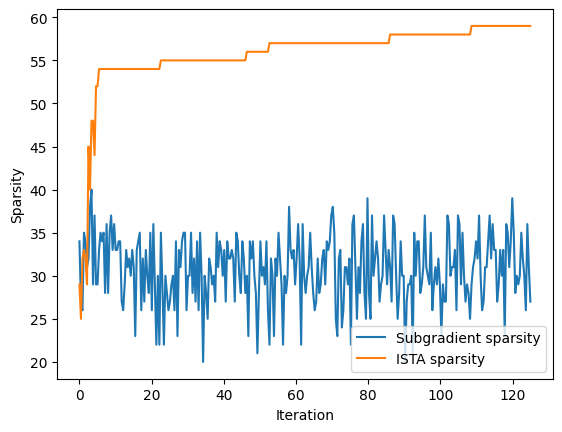
\includegraphics[width=\textwidth]{figures/fig5.png}
        \caption{2.5 Sparsity under different $\lambda$ values}
    \end{subfigure}
    \hfill
    \begin{subfigure}[t]{0.32\textwidth}
        \centering
        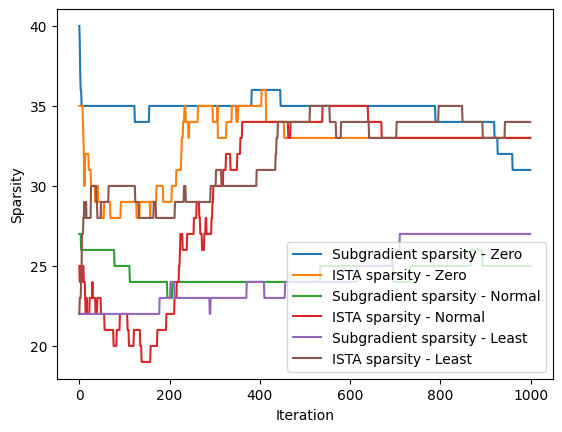
\includegraphics[width=\textwidth]{figures/fig6.png}
        \caption{2.5 Sparsity under different initializations}
    \end{subfigure}
    \hfill
    \begin{subfigure}[t]{0.32\textwidth}
        \centering
        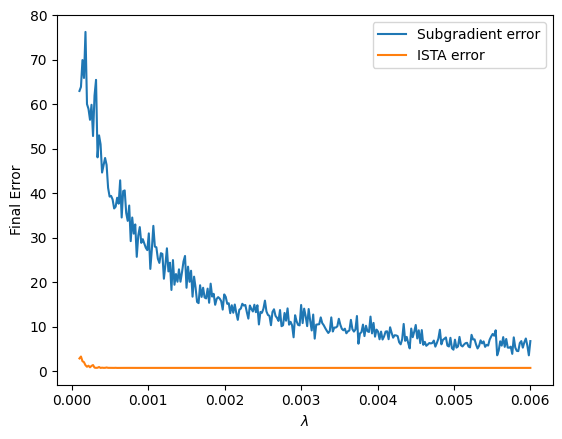
\includegraphics[width=\textwidth]{figures/fig7.png}
        \caption{2.7 Error under varying learning rates}
    \end{subfigure}
    \label{fig:three-inline}
\end{figure}

\subsection{Application to Boston Housing Data}

Finally, we apply both ISTA and SubGradient Descent to the Boston Housing dataset. The
target is the median house price.
As shown in the figure, ISTA achieves much faster convergence in training loss than SubGradient Descent, which aligns with our earlier synthetic results.
\subsection{Elastic Net}
We further extend our comparison to evaluate Elastic Net, which combines both $\ell_1$ and $\ell_2$ regularization. We optimize it using subgradient descent and compare it to SubGradient and ISTA. Results show that Elastic Net achieves faster convergence than SubGradient, highlighting its balanced regularization effect.

\begin{figure}[H]
    \centering
    \begin{subfigure}[t]{0.23\textwidth}
        \centering
        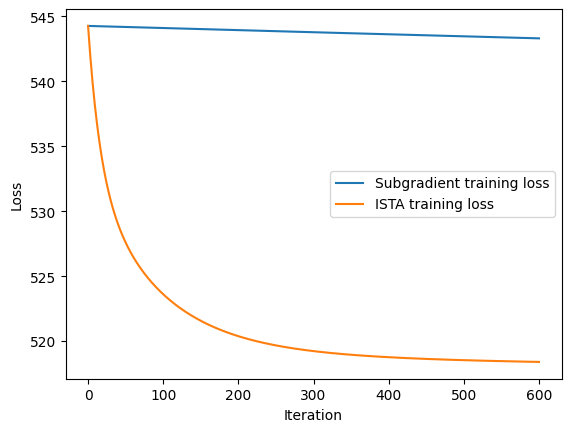
\includegraphics[width=\textwidth]{figures/fig8.png}
        \caption{2.8 Training loss comparison between SubGradient and ISTA}
    \end{subfigure}
    \hfill
    \begin{subfigure}[t]{0.23\textwidth}
        \centering
        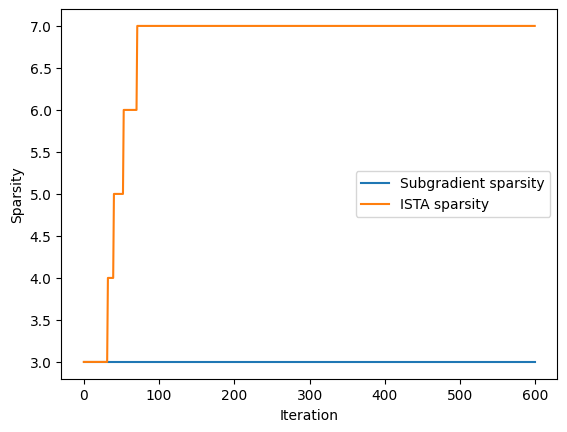
\includegraphics[width=\textwidth]{figures/fig9.png}
        \caption{2.9 Sparsity evolution of SubGradient and ISTA}
    \end{subfigure}
    \hfill
    \begin{subfigure}[t]{0.23\textwidth}
        \centering
        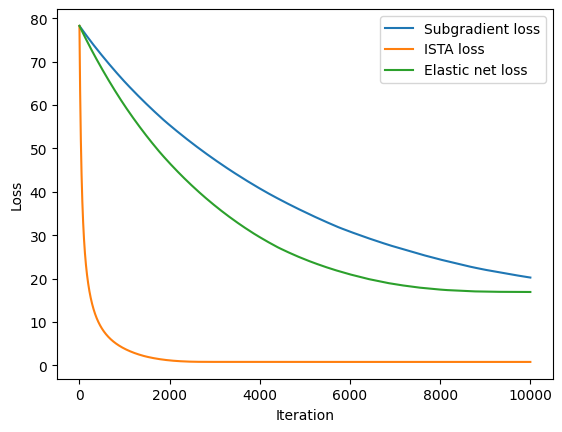
\includegraphics[width=\textwidth]{figures/fig10.png}
        \caption{2.10 Loss comparison among SubGradient, ISTA and Elastic Net}
    \end{subfigure}
    \hfill
    \begin{subfigure}[t]{0.23\textwidth}
        \centering
        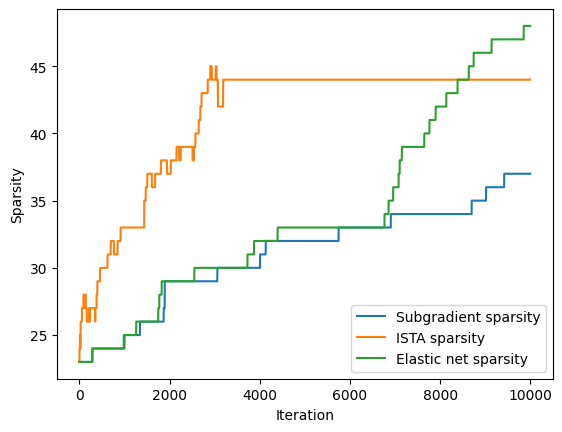
\includegraphics[width=\textwidth]{figures/fig11.png}
        \caption{2.11 Sparsity comparison among SubGradient, ISTA and Elastic Net}
    \end{subfigure}

    \label{fig:four-in-a-row}
\end{figure}

\section{Discussion}
Our results show that ISTA consistently outperforms SubGradient Descent in convergence speed and sparsity, and is more robust to initialization and learning rates. Elastic Net also improves performance over SubGradient when input features are correlated, balancing sparsity and stability through combined $\ell_1$-$\ell_2$ regularization. These results highlight the effectiveness of structured optimization in sparse regression. However, our experiments are limited by fixed hyperparameters, synthetic data, and lack of test-set validation. Future work could explore adaptive tuning, generalization to larger and noisier datasets, and model selection via cross-validation.

\end{document}